\documentclass[border=6pt]{standalone}
% Shared preamble for web figures.  Each figure is a standalone .tex that
% \input's this file; scripts/make-figures.sh turns it into an SVG.
% Handouts pull the same file with \fig{Unit_X/<name>}.
\usepackage[T1]{fontenc}
\usepackage{helvet}
\renewcommand{\familydefault}{\sfdefault}
\usepackage{amsmath}
\usepackage{tikz}
\usetikzlibrary{arrows.meta,positioning,calc,shapes.symbols,shapes.geometric}

% Who makes the rules is the point of most diagrams in this book, so the
% colors mean the same thing everywhere: blue is a person, orange is the
% computer, green is an answer, pink is the human brain.
\definecolor{person}{HTML}{2C6FAE}
\definecolor{machine}{HTML}{D35400}
\definecolor{result}{HTML}{1E8449}
\definecolor{brainpink}{HTML}{C2185B}
\definecolor{ink}{HTML}{2C3E50}

\tikzset{
  doodle/.style={line width=1.5pt, line cap=round, line join=round, draw=ink},
  box/.style={draw, rounded corners=5pt, line width=1.1pt, align=center,
              inner sep=7pt, minimum height=1.0cm, font=\small},
  personbox/.style={box, draw=person, fill=person!10},
  machinebox/.style={box, draw=machine, fill=machine!10},
  resultbox/.style={box, draw=result, fill=result!10},
  plainbox/.style={box, draw=ink!70, fill=ink!4},
  flow/.style={-{Stealth[length=8pt]}, line width=1.4pt, draw=ink},
}

\begin{document}
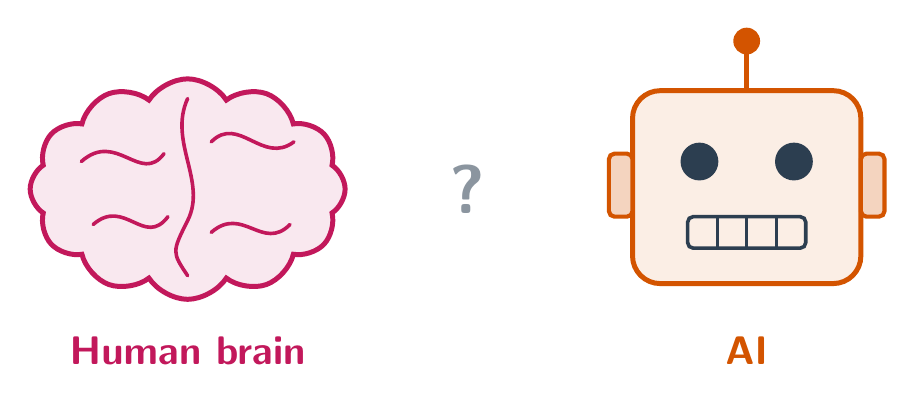
\begin{tikzpicture}
% The question that runs through the whole class.

% brain
\node[cloud, cloud puffs=12, cloud puff arc=115, aspect=1.45, draw=brainpink, fill=brainpink!10,
      line width=1.8pt, minimum width=4.0cm, minimum height=2.8cm] at (0,0) {};
\draw[brainpink, line width=1.3pt, line cap=round]
  (0,1.15) .. controls (-0.25,0.6) and (0.25,0.1) .. (0,-0.4) .. controls (-0.2,-0.8) .. (0,-1.1)
  (-1.35,0.35) .. controls (-0.9,0.75) and (-0.6,0.05) .. (-0.3,0.45)
  (-1.2,-0.45) .. controls (-0.8,-0.1) and (-0.55,-0.75) .. (-0.25,-0.35)
  (0.3,0.6) .. controls (0.65,0.95) and (0.95,0.3) .. (1.35,0.6)
  (0.3,-0.55) .. controls (0.7,-0.2) and (0.95,-0.8) .. (1.3,-0.45);
\node[font=\Large\bfseries, text=brainpink] at (0,-2.05) {Human brain};

% question mark
\node[font=\fontsize{64}{64}\selectfont\bfseries, text=ink!55] at (3.55,0) {?};

% AI
\begin{scope}[xshift=7.1cm]
  \draw[machine, line width=1.8pt] (0,1.25) -- (0,1.75);
  \fill[machine] (0,1.88) circle (0.17);
  \draw[machine, line width=1.8pt, fill=machine!10, rounded corners=10pt] (-1.45,-1.2) rectangle (1.45,1.25);
  \draw[machine, line width=1.5pt, fill=machine!25, rounded corners=2pt] (-1.75,-0.35) rectangle (-1.45,0.45);
  \draw[machine, line width=1.5pt, fill=machine!25, rounded corners=2pt] (1.45,-0.35) rectangle (1.75,0.45);
  \fill[ink] (-0.6,0.35) circle (0.24);
  \fill[ink] (0.6,0.35) circle (0.24);
  \draw[ink, line width=1.3pt, rounded corners=2pt] (-0.75,-0.75) rectangle (0.75,-0.35);
  \foreach \x in {-0.375,0,0.375} \draw[ink, line width=1pt] (\x,-0.75) -- (\x,-0.35);
  \node[font=\Large\bfseries, text=machine] at (0,-2.05) {AI};
\end{scope}
\end{tikzpicture}
\end{document}
